% Created 2024-11-11 Mon 07:32
% Intended LaTeX compiler: lualatex
\documentclass{beamer}
\usetheme{default}
\author{fabio}
\date{\today}
\title{Isomeria Óptica}
\hypersetup{
 pdfauthor={fabio},
 pdftitle={Isomeria Óptica},
 pdfkeywords={},
 pdfsubject={},
 pdfcreator={Emacs 29.4 (Org mode 9.6.15)}, 
 pdflang={English}}
\begin{document}

\begingroup
  \setbeamertemplate{headline}{}
  \maketitle
  \endgroup
\begin{frame}{Sumário}
\tableofcontents
\end{frame}



\begin{frame}[label={sec:org50c07fd}]{Isomeria Ótica}
\begin{block}{Isomeria Óptica}
\begin{itemize}
\item Tipo de isomeria em que uma molécula é a imagem especular da outra.
\item Ocorre em moléculas que não apresentam plano de simetria (moléculas assimétricas).
\item \alert{Isômeros Óticos} ou \alert{Enantiomorfos} ou \alert{Enantiômeros}
\end{itemize}

\begin{bclogo}[couleur=blue!30 , arrondi=0.1 , logo=\bcplume , epBarre=3.5]{Definição}
\alert{Estereoisômeros} são substâncias que têm a mesma sequência de átomos ligados, mas que se diferenciam no arranjo espacial dos átomos. Eles também são chamados de isômeros configuracionais.
\end{bclogo}
\end{block}


\begin{block}{}
\begin{itemize}
\item Esta molécula não apresenta nenhum plano de simetria.
\item É denominada molécula assimétrica ou molécula \alert{quiral}.
\item Se a colocarmos diante de um espelho, a imagem especular será diferente dela.
\end{itemize}

\begin{center}
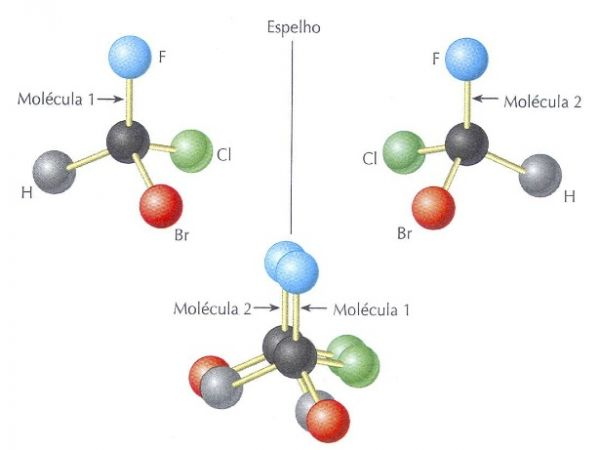
\includegraphics[scale=.5]{./Isomeria_Espelho.jpg}
\end{center}
\end{block}
\end{frame}



\begin{frame}[label={sec:org89949d2}]{Carbono Quiral}
\begin{block}{Carbono Quiral}
\begin{itemize}
\item Condição para haver isômeros óticos: presença de carbono \alert{quiral} ou \alert{assimétrico}
\end{itemize}

\begin{bclogo}[couleur=blue!30 , arrondi=0.1 , logo=\bcplume , epBarre=3.5]{Definição}

\end{bclogo}
\end{block}
\end{frame}


\begin{frame}[label={sec:org2aaad83}]{Isômeros Ópticos}
\begin{block}{Isômeros Ópticos}
Existem duas classes de isômeros ópticos:
\begin{itemize}
\item \alert{Enantiômeros}: estereoisômeros que são imagens especulares um do outro, que não se superpõem.
\end{itemize}

\begin{center}
\begin{tikzpicture}[thick,scale=1, every node/.style={scale=1}]
%\draw[help lines] (-10,-10) grid (10,10);
\tikzstyle{ground}=[fill,pattern=north east lines,draw=none,minimum width=0.3,minimum height=0.6]
%\node (wall1) [ground, minimum width=2cm] {};
\node (d1) [draw=none] at (-2,0){
\dtetrahedralS{0==C;1==COOH;2==CH$_{3}$;3A==H;4B==OH}};
\node (0,0) at (0,0) [ground,right= 1.5cm of d1, minimum height=2cm] (espelho) {};
\node (d2) [draw=none,right=.3cm] at (2,0){
\DtetrahedralS{0==C;1==COOH;2==CH$_{3}$;3A==H;4B==OH}};
\node (text1) [draw=none, below=0.2cm of d1, font=\bfseries] {$\mathcal{D}$-ácido lático};
\node (text2) [draw=none, below=0.2cm of d2, font=\bfseries] {$\mathcal{L}$-ácido lático};
\node (text3) [draw=none, red, above=0.2cm of espelho, font=\bfseries] {Espelho};
\end{tikzpicture}   
\end{center}

\begin{itemize}
\item As linhas normais (̶) representam os grupos que estão no plano do papel.
\item A linha tracejada representa o grupo que está atrás do plano.
\item A linha escura, em forma de cunha, representa o grupo que está na frente do plano do papel.
\end{itemize}
\end{block}


\begin{block}{}
\begin{itemize}
\item \alert{Diastereômeros}: estereoisômeros que não são imagens especulares um do outro e que não se superpõem.
\end{itemize}

\begin{center}
\begin{XyMcompd}(600,1150)(0,50){}{}
\tetrahedral{0==C;2B==Br;3A==H;4B==C$\ell$;%
1==\tetrahedral{0==C;3==(yl);2B==H$_3$C;4B==OH;1A==H}
}
\end{XyMcompd}
\hspace{1cm}
\begin{XyMcompd}(600,1150)(0,50){}{}
\tetrahedral{0==C;2B==Br;3A==H;4B==C$\ell$;%
1==\tetrahedral{0==C;3==(yl);2B==OH;4B==CH$_3$;1A==H}
}
\end{XyMcompd}
\end{center}
\end{block}
\end{frame}
\end{document}
